% ||||||||||||||||||||||||||||||||||||||||||||||
% Capitulo de Resultados Preliminares
% ||||||||||||||||||||||||||||||||||||||||||||||

\chapter{Análise de Resultados}

Neste capítulo são apresentados os resultados do projeto, os quais são os produtos dos estudos de casos desenvolvidos nas empresas parceiras.
Como se trata de um estudo de caso, e para as empresas, uma prova de conceito, os resultados também foram divididos por equipamento avaliado:
exaustor e seleira universal. Os mesmo, inicialmente são apresentados capturas de telas do software na parte de análise dos sinais coletados, para fim
de dar uma visão global do estado de saúde do equipamento no dado momento. Na sequência, gráficos específicos, levantando características e 
comparações em diferentes condições, mostrando a relação de causa e efeito. Por fim, apontamentos e discussões sobre os resultados de cada um
dos elementos, e também comparações entre os mesmos.

Para a apresentação dos resultados do exaustor, foram feitas capturas de tela do software do sistema que estava instalado no motor, de forma
remota e supervisionada pelos responsáveis pela manutenção dos mesmos. A Figura \ref{fig:exaustor_1} é a captura de tela do sistema no dia
em que um relatório sobre a saúde dos exautores foi gerado, com os dados daquele momento, e com os limites gerados pelo machine learning
no momento da instalação (06/12/2020).

\begin{figure}[H]
    \caption{Captura de tela do sistema instalado no exaustor.}
    \begin{center}
        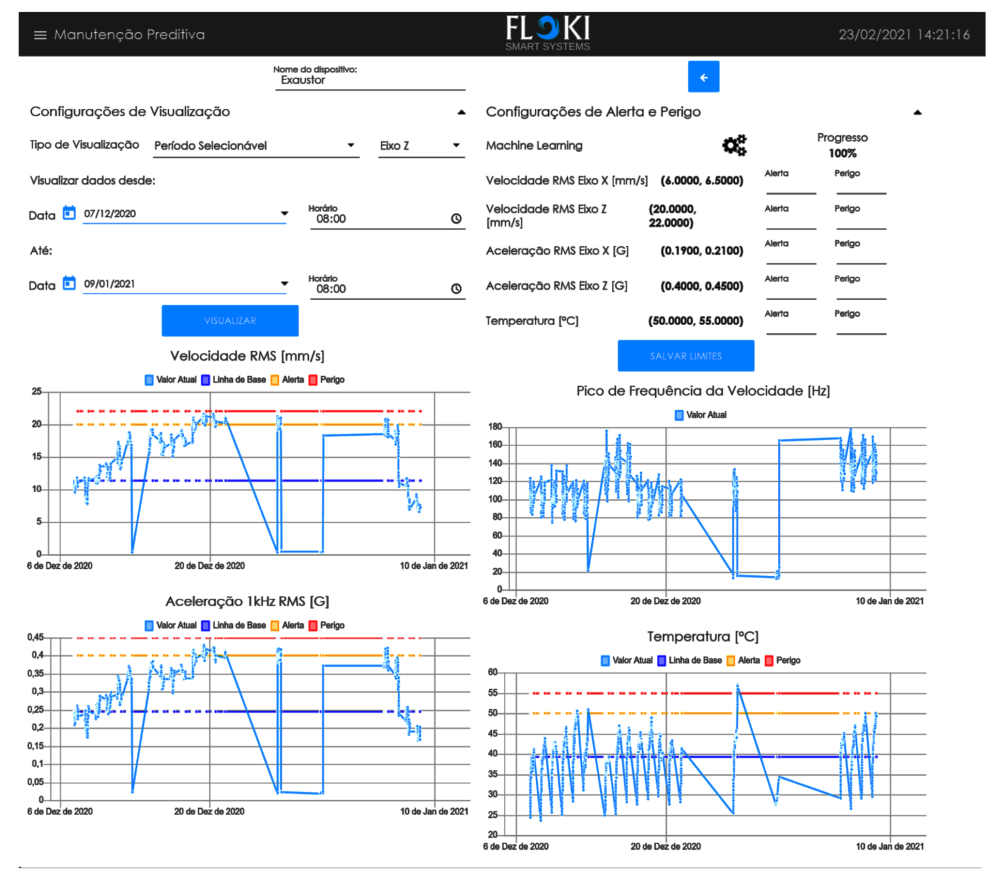
\includegraphics[scale=0.95, page=1]{resultados/img/resultados.pdf}
    \end{center}
    \fonte{Elaborado pelo Autor.} 
    \label{fig:exaustor_1}
\end{figure}

A captura de tela está com os dados de velocidade e aceleração do eixo Z, como podemos ver. Fica claro que as grandezas físicas
ultrapassam os limites estabelecidos pelo machine learning, somente no estado de alerta, mas isso não significa que o motor esteja em bom estado.
Se consultarmos a tabela \ref{tab:iso10816-1_randall_p146}, veremos que os valores para um motor de Classe I, segundo norma  ISO 10816-1, está 
entre apenas tolerável e não permitido, dependendo do regime de funcionamento. 
Se olharmos o eixo z, que se encontra na Figura \ref{fig:exaustor_xz}, os valores não permitidos, deixando claro o risco de falha iminente do 
motor.

\begin{figure}[H]
    \caption{Velocidade RMS [\SI{}{\milli\metre\per\second}] coletados do eixo x (A) e z (B).}
    \begin{center}
        \includegraphics[scale=0.65, page=2]{resultados/img/resultados.pdf}
    \end{center}
    \fonte{Elaborado pelo Autor.} 
    \label{fig:exaustor_xz}
\end{figure}

O eixo z se encontra em estado severo de vibração, não entrando em alarme devido ao machine learning tardio executado
pelo do operador, sendo agora uma tarefa de gestão do sistema, de se executar da maneira mais adequada, que é logo após o recondicionamento 
ou ajustar manualmente os limites de acordo com a norma ISO 10816-1. Outra característica importante é a temperatura, que pode ser vista na 
figura \ref{fig:exaustor_temperatura}, que teve uma dinâmica bem comportada e com característica de um sistema linear de primeira ordem.


\begin{figure}[H]
    \caption{Temperatura amostrada no exaustor.}
    \begin{center}
        \includegraphics[scale=0.65, page=3]{resultados/img/resultados.pdf}
    \end{center}
    \fonte{Elaborado pelo Autor.} 
    \label{fig:exaustor_temperatura}
\end{figure}

Fica nítido também o processo de aquecimento do dispositivo, seguindo os ciclos de funcionamento, que são bem regulares. O estudo de caso do 
exaustor se mostrou um ótimo caso para se analisar o comportamento do sistema em um dispositivo que já estava em funcionamento por um bom tempo 
após o recondicionamento, onde a técnica de machine learning, como esperado, não contribuiu com o objetivo de se detectar falhas, pois, as
condições iniciais não eram as ideais e os limites ficaram além dos permitidos. Mas o funcionamento geral da ferramenta foi excelente, sem nenhum
problema grave reportado, funcionando dentro das especificações e dentro do esperado pela empresa parceira. Um relatório foi gerado e entregue
para a empresa, contendo todos os dados e explicações, o qual foi aceito e sinalizaram o desejo de instalar em mais equipamentos.

A segunda prova de conceito foi realizada em uma seleira universal, como descrito anteriormente, onde 5 sensores foram distribuídos pela máquina, com o 
objetivo de monitorar os pontos críticos. Como no caso do exaustor, foram realizadas capturas de telas do sistema, onde a Figura
\ref{fig:seleira_universal} representa a captura dos dados do sensor 5, 4 dias antes de uma falha (08/12/2020). 

\begin{figure}[H]
    \caption{Linhas de base e sinais coletados em um dos 5 sensores na seleira universal.}
    \begin{center}
        \includegraphics[scale=0.9, page=4]{resultados/img/resultados.pdf}
    \end{center}
    \fonte{Elaborado pelo Autor.} 
    \label{fig:seleira_universal}
\end{figure}

Esta máquina não apresenta um processo contínuo como o exaustor, exigindo uma amostragem maior para se captar todas as características do 
funcionamento. Estes sensores foram instalados no dia 13/11/2020, mas os dados começaram a ser coletados apenas no dia 16/11/2020, onde a 
ferramenta de machine learning fui usada e os limites foram criados. 
A ferramenta foi aplicada em todos os 5 sensores, que foram instalados em acoplamentos, nas proximidades de polias e moto-redutores.
Cada um destes monitorou um comportamento diferente, mas o sensor mais importante se mostrou ser o 5, onde os resultados foram mais nítidos. 
Os outros sensores, pelo menos mais 3 apresentaram comportamento anômalos, mas nenhum como este. A Figura \ref{fig:seleira_universal_antes_depois}
apresenta uma comparação dos dados de velocidade logo após a instalação, com os dados na iminência de uma falha.

\begin{figure}[H]
    \caption{Linhas de base e dados de velocidade [\SI{}{\milli\metre\per\second} no momento da instalação
    (A) x próximo da falha (B).}
    \begin{center}
        \includegraphics[scale=0.65, page=5]{resultados/img/resultados.pdf}
    \end{center}
    \fonte{Elaborado pelo Autor.} 
    \label{fig:seleira_universal_antes_depois}
\end{figure}

Como podemos ver, os dados coletados na iminência da falha ultrapassam os limites de alerta e perigo, mesmo que não continuamente, mas
como a regra estabelecida na metodologia, da existência de 5 picos ou média acima dos limites, caracterizando uma alerta. Como são muitos dados,
um a cada $\SI{30}{\second}$, a visualização das retas de limites ficam comprometidas, e só é possível ver pela parte da tela onde se edita os
valores, ou pelos pontos azuis-escuros, amarelos e vermelhos no lado direito do gráfico. Além disso, é possível notar que no início do processo,
o sistema já se encontrava em uma situação pouco tolerável, segundo a norma ISO 10816-1, justificável por estarem instalados em partes que 
normalmente vibram mais, justamente por possuírem muitos elementos mecânicos e partes móveis. Por fim, a seleira universal apresentou o rompimento de uma
correia alguns dias após estes dados serem coletados e visualmente alertar uma condição severa de falha, consolidando o uso da ferramenta em
mais um equipamento, independente de ser um motor ou outro sistema mecânico. A aplicação funcionou perfeitamente, similar ao estudo de caso do
exaustor, apresentando apenas uma falha de salvar repetidas vezes os limites, que foi resolvida remotamente e incorporada ao software do projeto.
Uma peculiaridade de um sistema mancalizado, que difere de uma instalação em um motor elétrico de indução, é o comportamento da temperatura,
que pode ser visto na Figura \ref{fig:seleira_universal_temperatura}. 
Ela tem um perfil mais discreto, e não seguindo um sistema de primeira ordem, por não estar próximo de uma fonte de calor significativa, por isso
os limites gerados para algo com pouca variância, são limites muito próximos dos dados amostrados, ocorrendo falsos positivos apenas com a
variação da temperatura ambiente. A solução para isso, já prevista no início do projeto, é a possibilidade do operador alterar os limites, de 
acordo com a dinâmica que o sistema está inserido, não cabendo utilizar  machine learning onde há pouca variância ou o equipamento já se 
encontra em severo desgaste. 

\begin{figure}[H]
    \caption{Temperatura [\SI{}{\celsius}] amostrada na seleira universal.}
    \begin{center}
        \includegraphics[scale=0.8, page=6]{resultados/img/resultados.pdf}
    \end{center}
    \fonte{Elaborado pelo Autor.} 
    \label{fig:seleira_universal_temperatura}
\end{figure}

Após a escrita de todo o trabalho, indo desde o conhecimento mínimo para o entendimento das propostas, passando pela descrição dos métodos
empregados, até a análise dos resultados, foi possível ver o funcionamento satisfatório do projeto. O próximo capítulo apresenta as conclusões
gerais do projeto, com os trabalhos futuros.